% chktex-file 8
% chktex-file 24
% chktex-file 36
\section{Đối tượng \texttt{std::atomic} trong C++}

Thư viện chuẩn C++ cung cấp lớp mẫu \texttt{std::atomic} nhằm hỗ trợ các thao tác truy cập dữ liệu nguyên tử trong môi trường đa luồng~\cite{cppreference_atomic, williams2019cppconcurrency}. Một thao tác nguyên tử là thao tác được thực hiện như một đơn vị không thể bị chia cắt, bảo đảm rằng các luồng khác không thể quan sát trạng thái trung gian của dữ liệu trong quá trình thực thi. Nhờ đó, \texttt{std::atomic} được sử dụng rộng rãi để xây dựng các cơ chế đồng bộ hóa không khóa (lock-free synchronization), giúp giảm chi phí đồng bộ hóa và cải thiện hiệu năng của chương trình.

Đối tượng \texttt{std::atomic} được khai báo dưới dạng lớp mẫu với kiểu dữ liệu cơ sở là một kiểu nguyên thủy hoặc kiểu có thể sao chép đơn giản. Ví dụ, đoạn mã trong Liệt kê~\ref{lst:atomic_declare} minh họa cách khai báo một biến nguyên tử kiểu số nguyên.

\begin{lstlisting}[language=C++,caption={Khai báo đối tượng atomic},label={lst:atomic_declare}]
#include <atomic>

std::atomic<int> counter(0);
\end{lstlisting}

Khác với các biến thông thường, việc truy cập dữ liệu của đối tượng \texttt{atomic} thường được thực hiện thông qua các hàm thành viên chuyên biệt. Một số thao tác phổ biến bao gồm~\cite{cppreference_atomic}:

\begin{itemize}
\item \textbf{\texttt{load()}:} Đọc giá trị hiện tại của đối tượng nguyên tử.

\item \textbf{\texttt{store()}:} Ghi một giá trị mới vào đối tượng nguyên tử.

\item \textbf{\texttt{exchange()}:} Thay thế giá trị hiện tại bằng giá trị mới và trả về giá trị trước khi thay thế.

\item \textbf{Các thao tác \texttt{compare\_exchange}:} So sánh giá trị hiện tại với giá trị kỳ vọng. Hai biến thể phổ biến là \nolinkurl{compare_exchange_weak()} và \nolinkurl{compare_exchange_strong()}; nếu hai giá trị bằng nhau thì cập nhật giá trị mới, ngược lại trả về giá trị hiện tại.
\end{itemize}

Ví dụ trong Liệt kê~\ref{lst:atomic_ops} minh họa việc sử dụng một số thao tác nguyên tử cơ bản.

\begin{lstlisting}[language=C++,caption={Các thao tác nguyên tử phổ biến},label={lst:atomic_ops}]
std::atomic<int> value(10);

int current = value.load();

value.store(20);

int old_value = value.exchange(30);

int expected = 30;
bool result = value.compare_exchange_strong(expected, 40);
\end{lstlisting}

Trong các chương trình thực tế, kết quả của các thao tác nguyên tử thường được sử dụng trực tiếp trong các biểu thức điều kiện để điều khiển luồng thực thi. Do đó, việc hỗ trợ nhận diện và xử lý các đối tượng \texttt{atomic} có vai trò quan trọng đối với các công cụ kiểm thử tự động. Nếu không mô hình hóa chính xác các thao tác như \texttt{load()}, \texttt{store()} hoặc \texttt{compare\_exchange()}, công cụ sẽ gặp khó khăn trong việc xây dựng dữ liệu kiểm thử và đánh giá độ phủ đối với các nhánh mã phụ thuộc vào trạng thái của biến nguyên tử.

\section{Kiểm thử đơn vị}

Kiểm thử đơn vị (Unit Testing) là quá trình kiểm tra tính đúng đắn của các đơn vị chức năng nhỏ nhất trong chương trình, chẳng hạn như hàm hoặc phương thức~\cite{phamngochung2014testing}. Mỗi lần kiểm thử được thực hiện thông qua một hoặc nhiều ca kiểm thử (Test Case), bao gồm dữ liệu đầu vào, điều kiện thực hiện và kết quả mong đợi. Mục tiêu của kiểm thử đơn vị là phát hiện sớm các lỗi logic trong quá trình phát triển, từ đó nâng cao chất lượng và độ tin cậy của phần mềm. Để đánh giá hiệu quả của bộ kiểm thử, người ta thường sử dụng các chỉ số độ phủ mã nguồn (Code Coverage), phản ánh mức độ mà mã nguồn đã được thực thi bởi các ca kiểm thử. Ba tiêu chí phổ biến là độ phủ câu lệnh (Statement Coverage), đo tỷ lệ số câu lệnh đã được thực thi ít nhất một lần, và độ phủ nhánh (Branch Coverage) và MC/DC (Modified condition/decision coverage), đo tỷ lệ các nhánh điều kiện đã được kiểm thử. Trong phạm vi đề tài này, độ phủ câu lệnh, độ phủ nhánh và MC/DC được sử dụng để đánh giá hiệu quả hỗ trợ kiểm thử đối với các chương trình sử dụng đối tượng \texttt{std::atomic}.


\section{Tổng quan dự án AKAUTAUTO}

AKAUTAUTO là công cụ hỗ trợ kiểm thử đơn vị tự động cho các chương trình C/C++, được phát triển bởi Phòng thí nghiệm Đảm bảo chất lượng phần mềm, Trường Đại học Công nghệ - Đại học Quốc gia Hà Nội, phối hợp cùng đơn vị FPT Global Automotive \& Manufacturing (FPT-GAM). Mục tiêu của dự án là hỗ trợ người kiểm thử xây dựng và thực thi các ca kiểm thử một cách hiệu quả, từ đó nâng cao chất lượng phần mềm và giảm chi phí kiểm thử thủ công.

Hệ thống được xây dựng dựa trên kỹ thuật thực thi tượng trưng động, kết hợp giữa thực thi cụ thể và phân tích tượng trưng để khám phá các đường thực thi trong chương trình~\cite{nguyenducanh2015,sen2005cute}. Thông qua việc phân tích mã nguồn C/C++, công cụ có khả năng xây dựng mô hình chương trình, thu thập các điều kiện rẽ nhánh, tạo dữ liệu kiểm thử và đánh giá độ phủ mã nguồn của các ca kiểm thử đã thực hiện.

Kiến trúc của AKAUTAUTO bao gồm nhiều thành phần chức năng liên kết với nhau. Đầu tiên, mã nguồn được phân tích bằng bộ phân tích cú pháp để xây dựng Cây cú pháp trừu tượng (Abstract Syntax Tree - AST) và các cấu trúc biểu diễn chương trình liên quan. Từ AST, hệ thống trích xuất thông tin về hàm cần kiểm thử, tham số đầu vào, kiểu dữ liệu và các điều kiện điều khiển luồng thực thi. Tiếp theo, công cụ xây dựng cây dữ liệu kiểm thử (Data Tree) nhằm biểu diễn các biến đầu vào dưới dạng cấu trúc có thể cấu hình và quản lý. Dựa trên thông tin thu thập được, hệ thống sinh mã kiểm thử (test driver), biên dịch chương trình và thực thi các ca kiểm thử tương ứng.

Ngoài khả năng hỗ trợ sinh dữ liệu kiểm thử, AKAUTAUTO còn cung cấp các chức năng đánh giá kết quả thực thi và hiển thị trực quan các vùng mã nguồn đã hoặc chưa được kiểm thử. Những thông tin này giúp người phát triển xác định các khu vực cần bổ sung dữ liệu kiểm thử để nâng cao chất lượng kiểm thử tổng thể.

Qua nhiều giai đoạn phát triển, AKAUTAUTO đã hỗ trợ nhiều kiểu dữ liệu và cơ chế kiểm thử khác nhau trong ngôn ngữ C/C++. Tuy nhiên, một số kiểu dữ liệu đặc biệt của thư viện chuẩn C++, chẳng hạn như \texttt{std::atomic}, vẫn chưa được hỗ trợ đầy đủ trong mô hình dữ liệu và quy trình kiểm thử của hệ thống. Đây cũng chính là động lực cho nghiên cứu mở rộng được trình bày trong báo cáo này.


\section{Mô hình node dữ liệu cho các cấu trúc dữ liệu chuẩn \texttt{STL} trong AKAUTAUTO}

Trong AKAUTAUTO, dữ liệu kiểm thử được biểu diễn dưới dạng cây dữ liệu, trong đó mỗi nút mô tả một biến, một trường dữ liệu hoặc một thành phần con của đối tượng cần kiểm thử. Đối với các kiểu dữ liệu cơ bản như \texttt{int}, \texttt{float}, \texttt{char} hoặc \texttt{bool}, hệ thống có thể biểu diễn trực tiếp thông qua các nút dữ liệu giá trị. Tuy nhiên, với các kiểu dữ liệu phức tạp hơn, đặc biệt là các kiểu thuộc thư viện chuẩn C++ như \texttt{std::vector}, \texttt{std::string} hoặc \texttt{std::map}, việc biểu diễn trực tiếp dưới dạng một giá trị đơn lẻ là không phù hợp. Do đó, AKAUTAUTO sử dụng mô hình \texttt{STLDataNode} để mô tả các đối tượng thuộc Standard Template Library (STL).

\texttt{STLDataNode} đóng vai trò là lớp biểu diễn trung gian cho các kiểu dữ liệu STL trong cây dữ liệu kiểm thử. Thay vì coi một đối tượng STL là một biến nguyên thủy, hệ thống phân rã đối tượng đó thành các thành phần có thể quản lý được, chẳng hạn như kích thước container, kiểu phần tử và danh sách các phần tử con. Cách biểu diễn này giúp người dùng có thể quan sát, cấu hình và nhập dữ liệu kiểm thử cho các đối tượng STL thông qua giao diện cây dữ liệu.

Ví dụ, với một biến kiểu \texttt{std::vector<int>}, hệ thống không chỉ lưu thông tin rằng biến có kiểu \texttt{std::vector<int>}, mà còn cần xác định số lượng phần tử và tạo ra các nút con tương ứng với từng phần tử trong vector. Mỗi phần tử con sau đó có thể được biểu diễn bằng một nút dữ liệu giá trị kiểu \texttt{int}. Nhờ đó, quá trình sinh test driver có thể khởi tạo lại đối tượng \texttt{std::vector<int>} bằng các giá trị mà người dùng đã cung cấp.

\begin{lstlisting}[language=C++,caption={Ví dụ khai báo đối tượng STL},label={lst:stl_vector_example}]
#include <vector>

void foo(std::vector<int> values) {
    if (values.size() > 0 && values[0] > 10) {
        // ...
    }
}
\end{lstlisting}

Với đoạn mã trên, cây dữ liệu kiểm thử có thể biểu diễn biến \texttt{values} như một nút \texttt{STLDataNode}. Nút này chứa thông tin về kiểu container là \texttt{std::vector}, kiểu phần tử là \texttt{int}, đồng thời quản lý các nút con tương ứng với từng phần tử của vector. Khi người dùng thiết lập kích thước và giá trị cho các phần tử, hệ thống có thể sinh mã khởi tạo tương ứng trong test driver.

\begin{lstlisting}[language=C++,caption={Ví dụ mã khởi tạo dữ liệu kiểm thử cho vector},label={lst:stl_vector_init}]
std::vector<int> values;
values.push_back(15);
\end{lstlisting}

Mô hình \texttt{STLDataNode} cho thấy cách AKAUTAUTO xử lý các kiểu dữ liệu không nguyên thủy bằng cách xây dựng một lớp biểu diễn riêng trong cây dữ liệu. Đây là cơ sở quan trọng để mở rộng hệ thống sang các kiểu dữ liệu đặc biệt khác. Trong phạm vi đề tài này, ý tưởng tương tự được áp dụng để xây dựng cơ chế hỗ trợ đối tượng \texttt{std::atomic}. Tuy nhiên, khác với các container STL, đối tượng \texttt{atomic} không biểu diễn một tập hợp phần tử mà bao bọc một giá trị cơ sở và cung cấp các thao tác truy cập nguyên tử như \texttt{load()}, \texttt{store()}, \texttt{exchange()} và \texttt{compare\_exchange()}. Vì vậy, việc hỗ trợ \texttt{atomic} cần một mô hình dữ liệu riêng, vừa kế thừa cách tổ chức của cây dữ liệu trong AKAUTAUTO, vừa bổ sung khả năng nhận diện kiểu dữ liệu cơ sở và sinh mã khởi tạo phù hợp cho đối tượng nguyên tử.

\section{Cây cú pháp trừu tượng trong phân tích mã nguồn C/C++}

Cây cú pháp trừu tượng (Abstract Syntax Tree - AST) là cấu trúc dạng cây biểu diễn thành phần cú pháp của chương trình sau quá trình phân tích mã nguồn~\cite{phamngochung2014ut}. Trong AST, mỗi nút tương ứng với một thành phần của chương trình, chẳng hạn như khai báo biến, lời gọi hàm, biểu thức điều kiện, câu lệnh gán hoặc định nghĩa hàm. So với mã nguồn dạng văn bản, AST giúp công cụ phân tích chương trình dễ dàng truy xuất thông tin về kiểu dữ liệu, tên biến, danh sách tham số và cấu trúc điều khiển.

Trong AKAUTAUTO, AST được sử dụng ở giai đoạn đầu của quy trình kiểm thử nhằm trích xuất thông tin cần thiết từ mã nguồn C/C++. Từ AST, hệ thống có thể xác định hàm cần kiểm thử, các tham số đầu vào, kiểu dữ liệu của từng biến và các biểu thức điều kiện xuất hiện trong thân hàm. Những thông tin này là cơ sở để xây dựng cây dữ liệu kiểm thử, sinh test driver và đánh giá độ phủ mã nguồn.

Đối với đề tài này, AST đóng vai trò quan trọng trong việc nhận diện các biến có kiểu \texttt{std::atomic}. Thay vì chỉ xử lý các kiểu dữ liệu cơ bản như \texttt{int}, \texttt{float} hoặc \texttt{bool}, hệ thống cần phân tích kiểu dữ liệu dạng mẫu như \texttt{std::atomic<T>} để xác định kiểu dữ liệu cơ sở \texttt{T}. Việc nhận diện chính xác kiểu \texttt{atomic} trong AST là bước đầu tiên để ánh xạ biến nguyên tử sang mô hình \texttt{AtomicDataNode} trong cây dữ liệu kiểm thử.

\section{Test driver và stub trong AKAUTAUTO}

Trong kiểm thử đơn vị, test driver là đoạn mã được sinh ra để khởi tạo dữ liệu đầu vào, gọi hàm cần kiểm thử và thu thập kết quả thực thi~\cite{nguyenducanh2015}. Đối với AKAUTAUTO, test driver được tạo tự động dựa trên cây dữ liệu kiểm thử do người dùng hoặc hệ thống thiết lập. Mỗi biến đầu vào trong Data Tree sẽ được chuyển thành các câu lệnh khai báo và khởi tạo tương ứng trong mã kiểm thử.

Bên cạnh test driver, stub được sử dụng để thay thế hoặc mô phỏng hành vi của các hàm phụ thuộc trong quá trình kiểm thử~\cite{trannguyenhuong2022stub}. Khi hàm cần kiểm thử gọi đến một hàm khác chưa được kiểm thử trực tiếp, hệ thống có thể sinh stub nhằm kiểm soát giá trị trả về hoặc trạng thái dữ liệu liên quan. Cơ chế này giúp cô lập đơn vị cần kiểm thử và giảm sự phụ thuộc vào các thành phần bên ngoài.

Trong ngữ cảnh hỗ trợ \texttt{std::atomic}, cả test driver và stub đều cần được điều chỉnh để sinh mã phù hợp với ngữ nghĩa của đối tượng nguyên tử. Khác với các biến thông thường, \texttt{std::atomic} không nên được xử lý bằng phép gán trực tiếp trong một số ngữ cảnh sinh mã. Thay vào đó, hệ thống cần sử dụng \texttt{store()} để ghi giá trị và \texttt{load()} để đọc giá trị hiện tại. Đây là cơ sở cho việc mở rộng cơ chế sinh mã kiểm thử và khắc phục lỗi biên dịch khi xử lý các tham số hoặc biến có kiểu \texttt{std::atomic}.

\section{Tổng quan về công cụ VectorCAST}

VectorCAST là một công cụ kiểm thử đơn vị thương mại dành cho các ngôn ngữ C và C++, được phát triển bởi Vector Software~\cite{vectorcast2025}. Công cụ hỗ trợ tự động xây dựng môi trường kiểm thử, sinh test driver, quản lý dữ liệu kiểm thử, thực thi test case và thu thập các chỉ số độ bao phủ mã nguồn như Statement Coverage, Branch Coverage, MC/DC và Function Coverage. Nhờ khả năng tích hợp với nhiều trình biên dịch và môi trường phát triển khác nhau, VectorCAST được sử dụng rộng rãi trong các lĩnh vực yêu cầu độ tin cậy cao như ô tô, hàng không và hệ thống nhúng.

Quy trình kiểm thử trong VectorCAST bắt đầu bằng việc lựa chọn đơn vị kiểm thử (Unit Under Test - UUT), sau đó công cụ phân tích mã nguồn để xây dựng mô hình dữ liệu của các tham số đầu vào, biến toàn cục và giá trị trả về. Dựa trên mô hình này, người dùng có thể tạo và quản lý các bộ dữ liệu kiểm thử thông qua giao diện đồ họa mà không cần viết mã kiểm thử thủ công.

Tuy nhiên, kết quả thực nghiệm cho thấy việc hỗ trợ các kiểu dữ liệu hiện đại của C++ vẫn còn một số hạn chế. Đối với kiểu dữ liệu \texttt{std::atomic<T>}, VectorCAST không tự động nhận diện và sinh dữ liệu kiểm thử tương ứng như đối với các kiểu nguyên thủy hoặc cấu trúc dữ liệu thông thường. Thay vào đó, tham số kiểu \texttt{std::atomic<T>} được hiển thị dưới dạng \textit{user-defined parameter} và yêu cầu người dùng tự cung cấp mã khởi tạo thông qua cơ chế \textit{User Code}. Điều này cho thấy công cụ chưa xây dựng được mô hình dữ liệu nội bộ cho đối tượng atomic và chưa hỗ trợ tự động sinh dữ liệu kiểm thử cho kiểu dữ liệu này.

Hình~\ref{fig:VectorCAST} minh họa trường hợp VectorCAST không thể tự động gán giá trị cho tham số kiểu \texttt{std::atomic<int>} và yêu cầu người dùng nhập mã khởi tạo thủ công.

\begin{figure}[H]
\centering
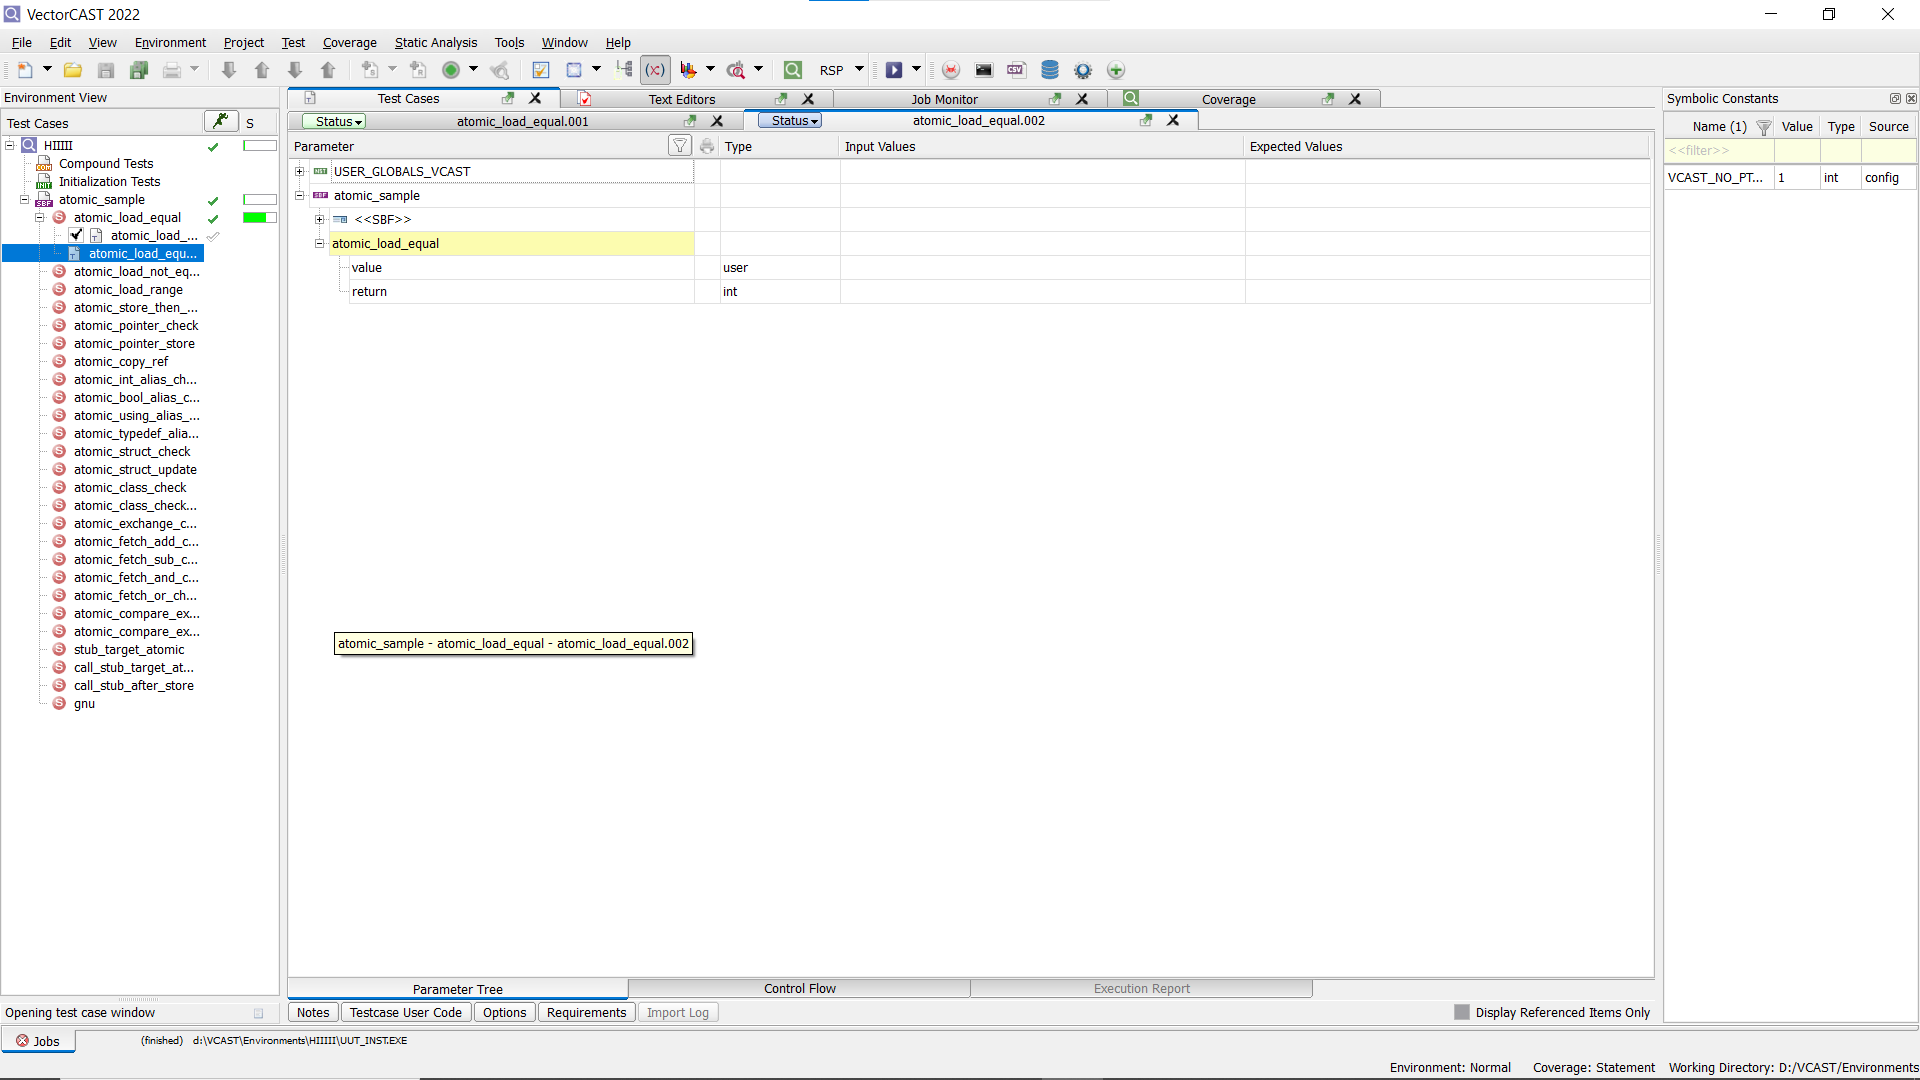
\includegraphics[width=0.9\linewidth]{images/VectorCAST.png}
\caption[VectorCAST yêu cầu nhập mã khởi tạo thủ công]{VectorCAST yêu cầu nhập mã khởi tạo thủ công cho tham số \texttt{std::atomic}}
\label{fig:VectorCAST}
\end{figure}